
\documentclass[conference]{IEEEtran}
\usepackage{graphicx,times,amsmath,colortbl, psfrag} % Add all your packages here
\usepackage[T1]{fontenc}
\usepackage[utf8]{inputenc}
\usepackage[spanish]{babel}
\usepackage[ruled, vlined, english, boxed, linesnumbered, lined]{algorithm2e}
%\renewcommand{\algorithmicrequire}{\textbf{Input:}}
%\renewcommand{\algorithmicensure}{\textbf{Output:}}
\usepackage{algpseudocode} 

\usepackage{multirow}

\usepackage {amsfonts}
\usepackage {amsmath}




% *** GRAPHICS RELATED PACKAGES ***
%\usepackage[pdftex]{graphicx}
%%
%\ifCLASSINFOpdf
%   
%  % declare the path(s) where your graphic files are
%   \graphicspath{{../pdf/}{../jpeg/}}
%  % and their extensions so you won't have to specify these with
%  % every instance of \includegraphics
%   \DeclareGraphicsExtensions{.pdf,.jpeg,.png}
%\else
%  \fi


\begin{document}
%
% paper title
% can use linebreaks \\ within to get better formatting as desired
\title{Pr\'actica 1. ``An\'alisis experimental de la eficiencia de algoritmos de ordenamiento''}


% author names and affiliations
% use a multiple column layout for up to three different
% affiliations
\author{\IEEEauthorblockN{Christian Miguel Hernández Mej\'ia}

\IEEEauthorblockA{
Departamento de Ciencias e Ingenier\'ia de la Computaci\'on,\\ 
An\'alisis de Algoritmos, ESCOM-IPN\\
 (email: christian.mhm@outlook.com)
}
}
% make the title area
\maketitle



\section{Introducci\'on}
El alumno realizar\'a un an\'alisis a posteriori de diversos algoritmos de ordenamiento. Implementar\'a y comparar\'a la eficiencia de estos algoritmos en los casos mejor, peor y promedio.

Para mostrar la eficiencia de diferentes algoritmos que solucionan un mismo problema, se consider\'o el problema de ordenamiento de una lista de n\'umeros enteros. Los algoritmos que se implementar\'an son:

\begin{enumerate}
	\item Ordenamiento por inseci\'on
	\item El m\'etodo de la burbuja 
	\item Ordenamiento por mezcla
	\item Ordenamiento r\'apido (Quick-sort)
\end{enumerate}

\section{Marco teórico}

\subsection{Algoritmo}

El término de algoritmo se puede entender como la descripción de cómo resolver un problema. El conjunto de instrucciones que especifican la secuencia de operaciones a realizar, en orden, para resolver un sistema específico o clase de problemas, también se denomina algoritmo. En otras palabras un algoritmo es una "especie de fórmula" para la resolución de un problema.

Además de ser un conjunto finito de reglas que dan lugar a una secuencia de operaciones para resolver un tipo específico de problema, un algoritmo debe cumplir cinco importantes condiciones:

\begin{enumerate}
\item Finitud. Un algoritmo tiene que acabar tras un número finito de pasos.
\item Definibilidad. Cada paso de un algoritmo debe de tener un significado preciso; las acciones a realizar han de estar especificadas en cada paso rigurosamente y sin ambigüedad.
\item Conjunto de entradas. Debe existir un conjunto específico de objetos, cada uno de los cuales constituye los datos iniciales de un caso particular del problema que resuelve el algoritmo. A este conjunto se llama conjunto de entrada del algoritmo.
\item Conjunto de salidas. Debe existir un conjunto específico de objetos, cada uno de los cuales constituye la salida o respuesta que debe tener el algoritmo para los diferentes casos particulares del problema. Para cada entrada del algoritmo debe existir una salida asociada.
\item Efectividad. Un algoritmo debe ser efectivo. Esto significa que todas las operaciones realizadas en el algoritmo deben ser lo bastante básicas para poder ser efectuadas de modo exacto en un lapso finito por el procesador.
\end{enumerate}

\subsection{An\'alisis a priori y posteriori}

El tiempo de ejecución de un algoritmo va a depender de diversos factores como son: los datos de entrada que le suministremos, la calidad del código generado por el compilador para crear el programa objeto, la naturaleza y rapidez de las instrucciones máquina del procesador concreto que ejecute el programa, y la complejidad intrínseca del algoritmo. Hay dos estudios posibles sobre el tiempo:



Deber\'a enviar al correo \href{miriam.pescador@gmail.com}, una carpeta comprimida con la implementaci\'on de los c\'odigos python y el reporte en formato latex y pdf.
El asunto del correo deber\'a decir "Practica 1 Analisis de Algoritmos [nombre completo del alumno comenzando con el apellido paterno]".
La carpeta debe tener el nombre del alumno (comenzando por apellido paterno).
La fecha l\'imite de entrega es el pr\'oximo Martes 5 de febrero de 2019 a las 10:00 pm. Por cada d\'ia de retraso se penalizar\'a al alumno con 15\% de la calificaci\'on obtenida. 
\subsection{An\'alisis del mejor y peor caso}

El reporte en latex debe considerar las siguientes secciones:

\begin{itemize}
\item Introducci\'on: descripci\'on sobre la implementaci\'on de la pr\'actica
\item Marco te\'orico. En esta secci\'on deber\'a poner los conceptos de:
\begin{itemize}
	\item Algoritmo
	\item An\'alisis a priori y posteriori
	\item An\'alisis del mejor y peor caso
	\item Caso promedio
\end{itemize}
Incluya la bibliograf\'ia que fue consultada (use el formato de ejemplo para agregarlo a su reporte).
\item Implementaci\'on. Coloque en esta secci\'on los algoritmos proporcionados en la plantilla de latex. Proporcione informaci\'on sobre las caracter\'isticas del equipo de c\'omputo donde realiz\'o las pruebas (sistema operativo, tipo de procesador, memoria, etc.).
Adem\'as deber\'a documentar las bibliotecas que empleo para la implementaci\'on de los algoritmos.
\item Resultados. Incluya la tabla de resultados y graficas solicitadas.
\item Conclusiones. Describa cu\'ales fueron los mejores algoritmos y para qu\'e casos y/o n\'umero de datos de entrada. Proporcione una justificaci\'on del por qu\'e se obtuvieron estos resultados. 
\end{itemize} 

\subsection{Caso promedio}

\begin{algorithm}[h]
%\hspace*{\algorithmicindent} \textbf{Input.} {A: conjunto de n\'umeros enteros} \\
%\hspace*{\algorithmicindent} \textbf{Output.} {A: lista ordenada de los n\'umeros enteros}
\KwData{A : list of sortable items}
\Begin{	
  InsertionSort(A){ \\
  
	\For{$ i \leftarrow 2$ to $n$}{
		$j \leftarrow   i - 1 $;\\
		\While{$j \geq 1 $ and $A[j] > A[j+1]$}{
			swap(A[j], A[j+1]);\\
			$j \leftarrow j-1$;\\		
		}
	}
	return A;	
}
}
\caption{Insertion Sort Algorithm}
\label{merge}
\end{algorithm}
\section{Implementaci\'on}
\begin{algorithm}[h]
%\Begin{	
  MergeSort(A, $p$, $r$){ \\
  
	\If{$p < r$}{
		$q \leftarrow   \lfloor (p+r)/2 \rfloor $;\\
		MergeSort(A, $p$, $q$);\\
		MergeSort(A, $q+1$, $r$);\\
		Merge(A, $p$, $q$, $r$);
	}
	return A;	
%}
}
\caption{Merge Sort Algorithm}
\label{merge}
\end{algorithm}
 
\section{Resultados}
\begin{algorithm}[h]
\KwData{A : list of sortable items}
\Begin{	
  $n \leftarrow length(A)$;\\
   \Repeat{not swapped}{
      $swapped \leftarrow false$;\\
      \For { $i \leftarrow 1$ to $n$}{
           \If {$A[i-1] > A[i]$} {
            swap(A[i-1], A[i]);\\
            $swapped \leftarrow true$;\\
            }
      }
      $n \leftarrow n - 1$;
   } 
   return A;	
}
\caption{Bubble Sort Algorithm}
\label{bubble}
\end{algorithm}
 

\begin{algorithm}[h]
%\Begin{	
  QuickSort(A, $p$, $r$){ \\
	\If{$p < r$}{
		$q \leftarrow   Partition(A, p, r)$;\\
		QuickSort(A, $p$, $q$);\\
		QuickSort(A, $q+1$, $r$);\\
		
	}
	return A;	
%}
}
\caption{Quick Sort Algorithm}
\label{quick}
\end{algorithm}


\begin{algorithm}[h]
%\Begin{	
 Partition(A, $p$, $r$){ \\
  $x \leftarrow A[p]$;\\
  $i \leftarrow p-1$
  $j \leftarrow r+1$
  \While{true}{
   	\Repeat{$A[j]\leq x$}{
      		$j \leftarrow j - 1$;\\
	 }
	 \Repeat{$A[j]\geq x$}{
      		$i \leftarrow i + 1$;\\
	 }
	 \If{i < j}{
	 	exchange $A[i] \leftrightarrow A[j] $;
	 }
	 \Else{return j;}
      		
    }	
}
\caption{Partition Algorithm}
\label{partition}
\end{algorithm}

\section{Conclusiones}


La figura \ref{fig:grafica} muestra el comportamiento de las funciones.

\begin{figure}
	\centering
	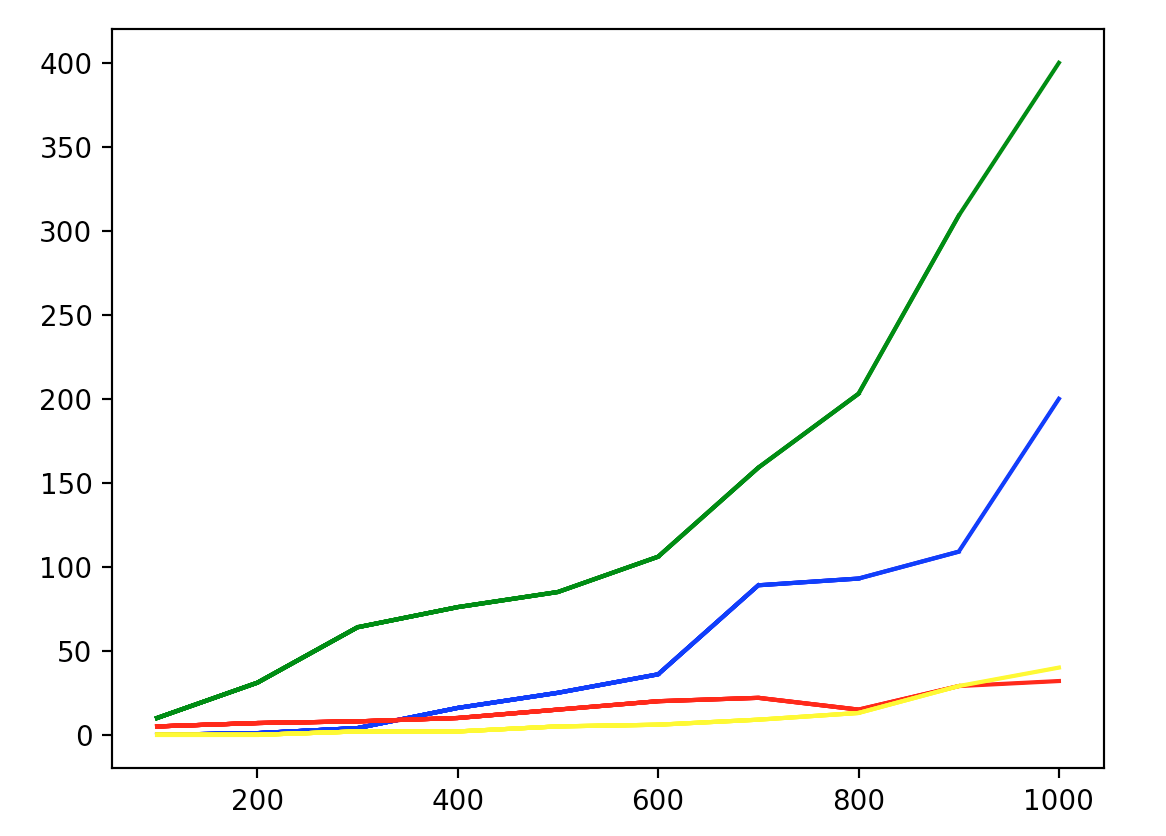
\includegraphics[width=1.0\columnwidth]{Imagenes/grafica1.png}
	\caption{Comparaci\'on del comportamiento de los algoritmos}
	\label{fig:grafica}
\end{figure}

%%%%%%%%%%%%%%%%%%%%%%%%%%%%%%%%%%%%%%%%%%%%%%%%%
\begin{table*}[!ht]
\begin{tabular}{|c|c|c|c|c|c|c|c|c|c|c|c|c|}
\hline
\multirow{2}{*}{n} & \multicolumn{4}{c|}{Mejor Caso} & \multicolumn{4}{c|}{Peor Caso} & \multicolumn{4}{c|}{Caso promedio} \\ 
\cline{2-13}
& insertion & merge & bubble & quick-sort & insertion & merge & bubble & quick-sort & insertion & merge & bubble & quick-sort \\ 
\hline
100 & 0.00004 & 0.00053 & 0.00002 & 0.00037 & 0.0043 & 0.00057 & 0.00317 & 0.00105 &0.00222 & 0.00053 & 0.00223 & 0.00038 \\
\hline
200 & 0.00007 & 0.00112 & 0.00004 & 0.00082 & 0.01701 & 0.00122 & 0.01415 & 0.00387 &0.00826 & 0.00111 & 0.00825 & 0.00084 \\
\hline
300 & 0.0001 & 0.00173 & 0.00006 & 0.00122 & 0.03562 & 0.00179 & 0.02891 & 0.00823 &0.0239 & 0.00275 & 0.01853 & 0.0013 \\
\hline
400 & 0.00015 & 0.00243 & 0.00008 & 0.00188 & 0.06773 & 0.00252 & 0.05509 & 0.0146 &0.03316 & 0.00243 & 0.03469 & 0.00197 \\
\hline
500 & 0.0002 & 0.00305 & 0.0001 & 0.00213 & 0.10576 & 0.00301 & 0.09013 & 0.02271 &0.05189 & 0.00317 & 0.05567 & 0.00249 \\
\hline
600 & 0.00026 & 0.00377 & 0.00013 & 0.00273 & 0.15838 & 0.00374 & 0.13153 & 0.03368 &0.07868 & 0.004 & 0.08355 & 0.00323 \\
\hline
700 & 0.00028 & 0.00448 & 0.00016 & 0.00342 & 0.21945 & 0.00486 & 0.17438 & 0.04396 &0.10799 & 0.00446 & 0.11606 & 0.00371 \\
\hline
800 & 0.00035 & 0.00519 & 0.00018 & 0.00401 & 0.26834 & 0.00562 & 0.23518 & 0.05862 &0.14652 & 0.00525 & 0.15862 & 0.00421 \\
\hline
900 & 0.0004 & 0.00586 & 0.00021 & 0.00437 & 0.35936 & 0.00645 & 0.29328 & 0.07464 &0.18821 & 0.00688 & 0.1986 & 0.00509 \\
\hline
1000 & 0.00041 & 0.00657 & 0.00023 & 0.00481 & 0.45372 & 0.0069 & 0.3641 & 0.09321 &0.22207 & 0.00686 & 0.23928 & 0.00636 \\
\hline
1100 & 0.00047 & 0.0073 & 0.00026 & 0.00531 & 0.53393 & 0.00772 & 0.46322 & 0.11531 &0.27688 & 0.00784 & 0.3133 & 0.00573 \\
\hline
1200 & 0.00054 & 0.00804 & 0.00028 & 0.006 & 0.6266 & 0.00848 & 0.55205 & 0.1391 &0.35499 & 0.00855 & 0.37082 & 0.00732 \\
\hline
1300 & 0.00058 & 0.00908 & 0.00033 & 0.00693 & 0.77711 & 0.0093 & 0.65278 & 0.16051 &0.39148 & 0.00961 & 0.43647 & 0.00749 \\
\hline
1400 & 0.00063 & 0.00992 & 0.00035 & 0.00765 & 0.89119 & 0.00981 & 0.76693 & 0.18674 &0.45845 & 0.01005 & 0.50069 & 0.00838 \\
\hline
1500 & 0.00068 & 0.01076 & 0.00037 & 0.00852 & 1.01579 & 0.01084 & 0.85042 & 0.21563 &0.51282 & 0.01021 & 0.56856 & 0.00874 \\
\hline
1600 & 0.00075 & 0.01154 & 0.00041 & 0.00879 & 1.12029 & 0.01168 & 0.98455 & 0.23823 &0.58039 & 0.01207 & 0.64386 & 0.00943 \\
\hline
1700 & 0.00081 & 0.01216 & 0.00042 & 0.00915 & 1.27038 & 0.01222 & 1.09936 & 0.26847 &0.68758 & 0.01176 & 0.71479 & 0.01017 \\
\hline
1800 & 0.00085 & 0.01274 & 0.00043 & 0.00981 & 1.45555 & 0.01262 & 1.25999 & 0.30539 &0.80086 & 0.01336 & 0.83244 & 0.01056 \\
\hline
1900 & 0.00087 & 0.01367 & 0.00047 & 0.00985 & 1.65317 & 0.0138 & 1.35414 & 0.34152 &0.84467 & 0.01377 & 0.91031 & 0.01162 \\
\hline
2000 & 0.0009 & 0.01419 & 0.00052 & 0.01056 & 1.86492 & 0.01434 & 1.57216 & 0.37403 &0.93678 & 0.01533 & 1.02076 & 0.01208 \\
\hline
2100 & 0.00096 & 0.01546 & 0.00052 & 0.01114 & 2.07778 & 0.01573 & 1.71545 & 0.41868 &0.98779 & 0.01629 & 1.10654 & 0.01237 \\
\hline
2200 & 0.00102 & 0.016 & 0.00055 & 0.0117 & 2.36808 & 0.01652 & 2.01138 & 0.46115 &1.10053 & 0.01711 & 1.21984 & 0.01308 \\
\hline
2300 & 0.00111 & 0.01678 & 0.0006 & 0.01277 & 2.60396 & 0.01714 & 2.14048 & 0.5326 &1.23108 & 0.01775 & 1.35991 & 0.01368 \\
\hline
2400 & 0.00104 & 0.01794 & 0.00058 & 0.01339 & 2.76839 & 0.01823 & 2.31622 & 0.53824 &1.3679 & 0.01853 & 1.5318 & 0.01471 \\
\hline
2500 & 0.0012 & 0.01957 & 0.00063 & 0.0138 & 3.07651 & 0.01884 & 2.5726 & 0.59267 &1.4527 & 0.021 & 1.61062 & 0.01582 \\
\hline
2600 & 0.00117 & 0.01917 & 0.00064 & 0.0145 & 3.20576 & 0.01963 & 2.79345 & 0.64369 &1.67686 & 0.0209 & 1.901 & 0.01603 \\
\hline
2700 & 0.0012 & 0.0199 & 0.00068 & 0.01549 & 3.54211 & 0.021 & 2.97286 & 0.69076 &1.80082 & 0.02003 & 2.01566 & 0.01705 \\
\hline
2800 & 0.00125 & 0.02083 & 0.0007 & 0.01624 & 3.6332 & 0.02109 & 3.12996 & 0.73518 &1.89767 & 0.02251 & 2.14826 & 0.01732 \\
\hline
2900 & 0.00122 & 0.02167 & 0.00076 & 0.01673 & 4.05976 & 0.0224 & 3.47323 & 0.78996 &2.01681 & 0.02359 & 2.23517 & 0.01819 \\
\hline
3000 & 0.00123 & 0.02239 & 0.00074 & 0.01804 & 4.06279 & 0.02239 & 3.50375 & 0.86524 &2.26116 & 0.02339 & 2.41566 & 0.01952 \\
\hline
3100 & 0.00127 & 0.02313 & 0.00075 & 0.01879 & 4.47494 & 0.02257 & 3.80297 & 0.90849 &2.35627 & 0.02403 & 2.61076 & 0.02265 \\
\hline
3200 & 0.00138 & 0.0242 & 0.00082 & 0.01911 & 4.7359 & 0.02463 & 4.0139 & 0.97525 &2.51247 & 0.0256 & 2.75704 & 0.02023 \\
\hline
3300 & 0.00153 & 0.02475 & 0.00081 & 0.01932 & 5.19063 & 0.02812 & 4.37771 & 1.04426 &2.65583 & 0.02644 & 2.96201 & 0.0207 \\
\hline
3400 & 0.00154 & 0.02571 & 0.00088 & 0.0201 & 5.40068 & 0.0248 & 4.39921 & 1.11152 &2.83969 & 0.0278 & 3.06315 & 0.0254 \\
\hline
3500 & 0.00155 & 0.02635 & 0.00085 & 0.02037 & 5.69257 & 0.02558 & 4.89481 & 1.15419 &3.11405 & 0.03025 & 3.3268 & 0.02127 \\
\hline
3600 & 0.00166 & 0.02729 & 0.00088 & 0.0212 & 6.32146 & 0.02756 & 5.40779 & 1.20714 &3.18333 & 0.03203 & 3.43907 & 0.02408 \\
\hline
3700 & 0.00162 & 0.02726 & 0.0009 & 0.02144 & 6.72922 & 0.02818 & 5.71833 & 1.29738 &3.35382 & 0.03001 & 3.82903 & 0.02388 \\
\hline
3800 & 0.00165 & 0.0296 & 0.00096 & 0.02221 & 7.01805 & 0.03037 & 5.77196 & 1.37338 &3.52107 & 0.03014 & 3.77971 & 0.02659 \\
\hline
3900 & 0.00179 & 0.02988 & 0.00095 & 0.02239 & 7.37257 & 0.0295 & 6.35707 & 1.45912 &3.68952 & 0.03225 & 4.11487 & 0.02469 \\
\hline
4000 & 0.00178 & 0.03053 & 0.00102 & 0.02311 & 7.84179 & 0.03104 & 6.74234 & 1.53608 &3.96538 & 0.03316 & 4.24705 & 0.03154 \\
\hline
4100 & 0.00171 & 0.0317 & 0.00104 & 0.02334 & 8.25381 & 0.03132 & 6.92144 & 1.54054 &4.20792 & 0.03848 & 4.50097 & 0.02815 \\
\hline
4200 & 0.0019 & 0.03234 & 0.00103 & 0.02425 & 8.73565 & 0.03246 & 7.27616 & 1.66007 &4.41867 & 0.03341 & 4.8266 & 0.0269 \\
\hline
4300 & 0.00171 & 0.03317 & 0.00113 & 0.02448 & 8.92524 & 0.03366 & 7.73239 & 1.7482 &4.54224 & 0.03428 & 4.93201 & 0.0295 \\
\hline
4400 & 0.00191 & 0.03417 & 0.00108 & 0.02544 & 9.63271 & 0.03536 & 8.23683 & 1.87839 &5.02727 & 0.0365 & 5.32899 & 0.03122 \\
\hline
4500 & 0.00192 & 0.03486 & 0.00116 & 0.02911 & 9.55284 & 0.0349 & 8.01894 & 1.90951 &4.9646 & 0.0359 & 5.39581 & 0.03057 \\
\hline
4600 & 0.00218 & 0.03495 & 0.00123 & 0.02688 & 10.11988 & 0.03633 & 8.54337 & 1.96109 &5.34844 & 0.03808 & 5.72692 & 0.03069 \\
\hline
4700 & 0.00194 & 0.03456 & 0.00113 & 0.02779 & 11.08914 & 0.03691 & 9.39998 & 2.12763 &5.61797 & 0.03763 & 5.83767 & 0.03039 \\
\hline
4800 & 0.00219 & 0.03628 & 0.00134 & 0.02834 & 11.16658 & 0.03783 & 9.4803 & 2.14118 &5.64035 & 0.0385 & 6.02284 & 0.03249 \\
\hline
4900 & 0.00227 & 0.03728 & 0.00126 & 0.02863 & 11.0089 & 0.03834 & 9.55177 & 2.22659 &6.02393 & 0.03948 & 6.46371 & 0.03479 \\
\hline
5000 & 0.00222 & 0.03849 & 0.00125 & 0.03006 & 12.28414 & 0.04086 & 10.1651 & 2.37931 &6.64304 & 0.04244 & 6.91255 & 0.03268 \\
\hline


\end{tabular}
\caption{Resultados de los tiempos de ejecuci\'on para cada algoritmo.}
\end{table*}


\begin{table*}[!ht]
\begin{tabular}{|c|c|c|c|c|c|c|c|c|c|c|c|c|}
\hline
\multirow{2}{*}{n} & \multicolumn{4}{c|}{Mejor Caso} & \multicolumn{4}{c|}{Peor Caso} & \multicolumn{4}{c|}{Caso promedio} \\ 
\cline{2-13}
& insertion & merge & bubble & quick-sort & insertion & merge & bubble & quick-sort & insertion & merge & bubble & quick-sort \\ 
\hline
5100 & 0.00237 & 0.03956 & 0.00135 & 0.03096 & 11.86569 & 0.03987 & 10.4662 & 2.42466 &6.72113 & 0.04133 & 7.03041 & 0.03421 \\
\hline
5200 & 0.00236 & 0.04077 & 0.00131 & 0.03315 & 13.30632 & 0.04147 & 11.21489 & 2.59864 &6.70386 & 0.0448 & 7.63108 & 0.03405 \\
\hline
5300 & 0.00213 & 0.04117 & 0.00134 & 0.03264 & 14.04131 & 0.04211 & 11.7817 & 2.70695 &7.17953 & 0.04307 & 7.47832 & 0.03957 \\
\hline
5400 & 0.00254 & 0.04234 & 0.00148 & 0.03314 & 13.94129 & 0.0412 & 11.6548 & 2.7586 &7.15353 & 0.04206 & 7.84451 & 0.03617 \\
\hline
5500 & 0.00253 & 0.0447 & 0.00147 & 0.03435 & 15.00754 & 0.04492 & 12.27709 & 2.95612 &7.6462 & 0.04493 & 8.26441 & 0.03911 \\
\hline
5600 & 0.00283 & 0.04385 & 0.00152 & 0.03478 & 15.552 & 0.04446 & 12.58985 & 3.0043 &7.92725 & 0.04559 & 8.38686 & 0.03853 \\
\hline
5700 & 0.00286 & 0.04309 & 0.00135 & 0.03518 & 15.69403 & 0.04464 & 13.50566 & 3.04532 &8.18756 & 0.04703 & 8.70768 & 0.0415 \\
\hline
5800 & 0.00251 & 0.04442 & 0.00159 & 0.037 & 16.68916 & 0.04683 & 14.2313 & 3.23257 &8.43192 & 0.04967 & 9.07723 & 0.04069 \\
\hline
5900 & 0.0023 & 0.04359 & 0.00157 & 0.03668 & 16.64704 & 0.04829 & 14.22058 & 3.43667 &9.44975 & 0.05082 & 9.4771 & 0.04164 \\
\hline
6000 & 0.00217 & 0.04554 & 0.00158 & 0.03845 & 17.01952 & 0.04752 & 14.54701 & 3.37739 &9.27645 & 0.04884 & 9.89645 & 0.0417 \\
\hline
6100 & 0.00247 & 0.04789 & 0.00172 & 0.04074 & 17.31442 & 0.04795 & 14.84847 & 3.59293 &9.07768 & 0.04807 & 9.71356 & 0.04136 \\
\hline
6200 & 0.0026 & 0.0486 & 0.00163 & 0.04097 & 18.12312 & 0.04911 & 15.50351 & 3.64618 &9.24071 & 0.05033 & 9.6437 & 0.04816 \\
\hline
6300 & 0.00262 & 0.04842 & 0.00157 & 0.04141 & 18.64095 & 0.05016 & 16.12714 & 3.93962 &9.27637 & 0.04902 & 9.95995 & 0.04188 \\
\hline
6400 & 0.00271 & 0.04996 & 0.00179 & 0.04151 & 19.37319 & 0.05058 & 16.47942 & 3.77345 &9.93631 & 0.05178 & 10.75847 & 0.04356 \\
\hline
6500 & 0.00262 & 0.04967 & 0.00177 & 0.04254 & 20.11301 & 0.05026 & 16.97366 & 3.96678 &10.03201 & 0.05224 & 10.75388 & 0.04442 \\
\hline
6600 & 0.00251 & 0.04976 & 0.00156 & 0.04275 & 20.34178 & 0.05639 & 17.85357 & 4.23023 &10.15059 & 0.05082 & 11.16921 & 0.0445 \\
\hline
6700 & 0.00265 & 0.0519 & 0.00181 & 0.04403 & 20.71048 & 0.05451 & 17.82014 & 4.23374 &10.95488 & 0.05369 & 11.63749 & 0.04889 \\
\hline
6800 & 0.00274 & 0.05208 & 0.00169 & 0.04384 & 21.66028 & 0.05441 & 18.50011 & 4.41793 &12.01144 & 0.05828 & 12.44916 & 0.04896 \\
\hline
6900 & 0.00298 & 0.05343 & 0.00165 & 0.04451 & 23.26109 & 0.05638 & 19.90725 & 4.57674 &12.01715 & 0.0581 & 12.53111 & 0.04671 \\
\hline
7000 & 0.00275 & 0.05329 & 0.00184 & 0.04507 & 22.72705 & 0.05628 & 19.63264 & 4.60645 &12.35293 & 0.05872 & 13.16561 & 0.04884 \\
\hline
7100 & 0.00286 & 0.0539 & 0.00184 & 0.04596 & 24.37205 & 0.05458 & 20.42626 & 4.86522 &12.25438 & 0.05876 & 13.35385 & 0.05756 \\
\hline
7200 & 0.0028 & 0.05526 & 0.00196 & 0.04779 & 24.18987 & 0.05807 & 20.61779 & 4.87488 &12.67942 & 0.05921 & 13.27246 & 0.05239 \\
\hline
7300 & 0.00309 & 0.05682 & 0.0018 & 0.04639 & 24.62426 & 0.0591 & 21.8431 & 5.27835 &13.45548 & 0.06206 & 13.8651 & 0.05063 \\
\hline
7400 & 0.00287 & 0.05816 & 0.00187 & 0.05104 & 27.16367 & 0.06561 & 22.8646 & 5.26104 &13.84587 & 0.06383 & 15.10167 & 0.05092 \\
\hline
7500 & 0.00278 & 0.05784 & 0.00198 & 0.04763 & 26.88516 & 0.05983 & 22.89381 & 5.27245 &14.18588 & 0.06187 & 14.6137 & 0.05062 \\
\hline
7600 & 0.00301 & 0.05918 & 0.0021 & 0.05059 & 28.53613 & 0.06141 & 24.12557 & 5.61043 &14.52791 & 0.06305 & 15.11816 & 0.05327 \\
\hline
7700 & 0.00319 & 0.05955 & 0.00203 & 0.04829 & 29.07954 & 0.06208 & 24.21112 & 5.74692 &14.98472 & 0.06421 & 16.19176 & 0.05556 \\
\hline
7800 & 0.00315 & 0.06092 & 0.00212 & 0.05033 & 28.44307 & 0.0653 & 24.41307 & 5.85094 &15.47308 & 0.06503 & 16.02677 & 0.05547 \\
\hline
7900 & 0.00342 & 0.06062 & 0.00208 & 0.04966 & 29.23592 & 0.06432 & 25.04833 & 5.9798 &15.18051 & 0.06604 & 16.16633 & 0.05313 \\
\hline
8000 & 0.00328 & 0.06111 & 0.00204 & 0.05005 & 30.75211 & 0.0643 & 25.97636 & 6.14224 &15.54448 & 0.06713 & 16.49118 & 0.05889 \\
\hline
8100 & 0.00332 & 0.06206 & 0.00201 & 0.0504 & 30.80202 & 0.0653 & 26.33753 & 6.31952 &15.97047 & 0.06769 & 16.45164 & 0.05775 \\
\hline
8200 & 0.00311 & 0.06295 & 0.00218 & 0.05198 & 31.72681 & 0.06687 & 27.08266 & 6.47782 &17.08102 & 0.07063 & 17.84501 & 0.05852 \\
\hline
8300 & 0.00327 & 0.06418 & 0.00218 & 0.05284 & 32.09278 & 0.0664 & 27.63708 & 6.65226 &15.92664 & 0.06819 & 17.13532 & 0.05827 \\
\hline
8400 & 0.00333 & 0.06778 & 0.00238 & 0.05333 & 33.99091 & 0.06932 & 28.27648 & 6.77881 &16.55687 & 0.06765 & 17.66588 & 0.06222 \\
\hline
8500 & 0.00326 & 0.0653 & 0.0021 & 0.05329 & 34.48587 & 0.06812 & 29.13349 & 6.88794 &18.1185 & 0.07688 & 18.79843 & 0.06655 \\
\hline
8600 & 0.00319 & 0.06568 & 0.00229 & 0.05437 & 35.8276 & 0.06928 & 29.91268 & 7.0183 &17.98148 & 0.07137 & 18.83774 & 0.05994 \\
\hline
8700 & 0.00349 & 0.06758 & 0.00224 & 0.05514 & 34.91012 & 0.07524 & 30.8944 & 7.26074 &18.34017 & 0.07231 & 19.09481 & 0.06238 \\
\hline
8800 & 0.00331 & 0.06791 & 0.00235 & 0.05574 & 36.11228 & 0.07296 & 30.76664 & 7.49378 &18.66354 & 0.07023 & 19.63803 & 0.06563 \\
\hline
8900 & 0.00338 & 0.07078 & 0.00235 & 0.05764 & 37.39638 & 0.07449 & 32.20866 & 7.60443 &19.18721 & 0.07371 & 20.34648 & 0.06249 \\
\hline
9000 & 0.00366 & 0.07034 & 0.00246 & 0.06042 & 38.28613 & 0.07523 & 32.41874 & 8.02558 &19.40703 & 0.07691 & 20.64081 & 0.06493 \\
\hline
9100 & 0.00355 & 0.07019 & 0.0024 & 0.05837 & 39.64623 & 0.07184 & 33.22122 & 8.14559 &20.0592 & 0.07584 & 21.11805 & 0.06683 \\
\hline
9200 & 0.00332 & 0.07164 & 0.00247 & 0.0593 & 40.91362 & 0.07271 & 34.31104 & 8.21484 &20.65041 & 0.07901 & 21.49568 & 0.06535 \\
\hline
9300 & 0.00352 & 0.0726 & 0.0025 & 0.05975 & 42.56315 & 0.07768 & 36.2567 & 8.41662 &21.53621 & 0.07729 & 22.80341 & 0.06688 \\
\hline
9400 & 0.00363 & 0.07372 & 0.00224 & 0.06057 & 42.47155 & 0.07475 & 36.24043 & 8.5558 &21.83496 & 0.08142 & 24.43336 & 0.06622 \\
\hline
9500 & 0.00351 & 0.07382 & 0.00237 & 0.06064 & 42.99277 & 0.0801 & 36.8555 & 8.49094 &22.48074 & 0.07989 & 24.18705 & 0.06998 \\
\hline
9600 & 0.00423 & 0.0751 & 0.00245 & 0.0603 & 45.39145 & 0.07999 & 37.42427 & 9.113 &22.76934 & 0.08092 & 24.22564 & 0.06824 \\
\hline
9700 & 0.00389 & 0.07531 & 0.00246 & 0.06426 & 45.52552 & 0.07937 & 39.15872 & 9.21488 &22.96866 & 0.08162 & 24.776 & 0.0689 \\
\hline
9800 & 0.00372 & 0.07562 & 0.00255 & 0.0641 & 45.653 & 0.08031 & 38.48726 & 9.41618 &23.71929 & 0.08264 & 25.46123 & 0.07142 \\
\hline
9900 & 0.00372 & 0.07643 & 0.00263 & 0.06566 & 46.11136 & 0.08125 & 39.65152 & 9.13532 &24.24912 & 0.08025 & 25.7858 & 0.08048 \\
\hline
10000 & 0.00363 & 0.07823 & 0.00258 & 0.06447 & 47.60412 & 0.07869 & 41.08169 & 9.64315 &24.6981 & 0.09382 & 25.66132 & 0.07198 \\
\hline


\end{tabular}
\caption{Resultados de los tiempos de ejecuci\'on para cada algoritmo.}
\end{table*}



\section{Referencias}


%\bibliography{my-paper}


% (used to reserve space for the reference number labels box)
\begin{thebibliography}{1}

\bibitem{moscato99}
P. Moscato,
\newblock {\em On evolution, search, optimization, genetic algorithms and martial arts: Towards memetic algorithms,}
\newblock  Technical Report C3P Report 826, 1989.

\bibitem{KrasnogorS00}%
N. Krasnogor and J. Smith,
\newblock {\em A Memetic Algorithm With Self-Adaptive Local Search: TSP as a case study,}
\newblock Genetic Evolutionary Computation Conference pp. 987-994, 2000. 

\end{thebibliography}

\end{document}


